\documentclass[0-protokol.tex]{subfiles}
\begin{document}
V této úloze jsou měřeny odpory šesti kovových drátů. Měříme-li hodnoty odporů menších než $\SI{1}{\ohm}$, do výsledků se začnou výrazně projevovat odpory vodičů měřicího zapojení. Tento jev eliminujeme pomocí \textit{čtyřbodového zapojení}, které je znázorněno na obrázku \ref{fig:ctyrbod}. Kontakty $a$ a $a'$ nazýváme proudové, $b$ a $b'$ napěťové.
\begin{figure}[H]
\centering
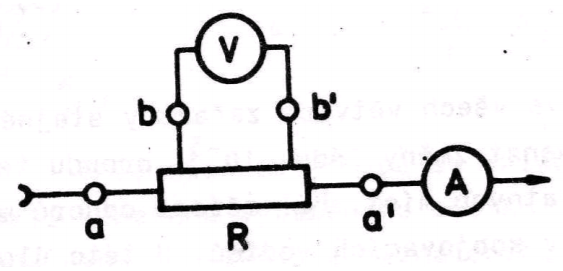
\includegraphics[scale=0.55]{ctyrbod}
\caption{Princip čtyřbodového zapojení \cite{stud_text}}
\label{fig:ctyrbod}
\end{figure}

Na obrázku \ref{fig:wheatstone} vidíme \textit{Wheatstoneův můstek}, který je vhodný pro měření odporů o velikosti $1$ - $\SI{e7}{\ohm}$, do měření malých odporů je však vnášena systematická chyba způsobená odpory vodičů. Při měření nastavujeme na odporové dekádě hodnoty odporu a při přepínání ručičky do polohy \textit{hrubě} či \textit{jemně} sledujeme výchylku galvanometru. Tu se snažíme minimalizovat. Měřený odpor získáme ze vztahu 
\begin{equation} \label{eq:wheatstone}
R_x = \frac{R_n}{1000},
\end{equation}
kde $R_n$ je odpor na dekádě. 
\begin{figure}[H]
\centering
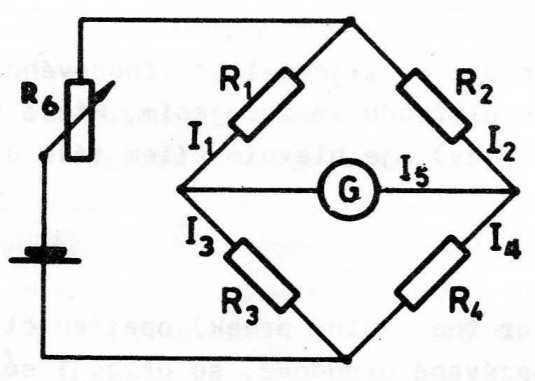
\includegraphics[scale=0.5]{wheatstone}
\caption{Zapojení Wheatstoneova můstku \cite{stud_text}}
\label{fig:wheatstone}
\end{figure}

Pro měření malých odporů je vhodnější využít \textit{Thomsonův můstek}, který eliminuje chybu způsobenou odporem vodičů. Zapojení Thomsonova můstku je znázorněno na obrázku \ref{fig:thomson}. Měření probíhá stejně jako v případě Wheatstoneova můstku, shodným vztahem získáme výsledný odpor.

Změříme-li odpor přívodních vodičů $R_V$ Wheatstoneovým můstkem, můžeme spočíst odpor na svorkách 
\begin{equation} \label{eq:svorky}
R_S = R_W - R_T - R_V,
\end{equation}
kde $R_W$ je odpor drátů měřený Wheatstoneovým a $R_T$ Thomsonovým můstkem.
\begin{figure}[H]
\centering
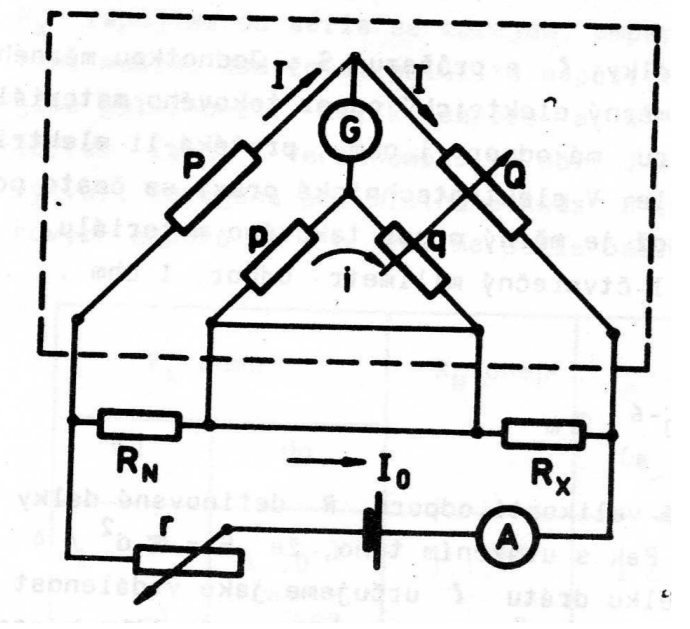
\includegraphics[scale=0.4]{thomson}
\caption{Zapojení Thomsonova můstku \cite{stud_text}}
\label{fig:thomson}
\end{figure}

Odpory kovových drátů změříme také pomocí multimetru \textbf{KEITHLEY 2010} za použití čtyřbodového zapojení. Schéma měření je zobrazeno na obrázku \ref{fig:keithley}. Před měřením stiskneme na multimetru tlačítko $\Omega 4$.
\begin{figure}[H]
\centering
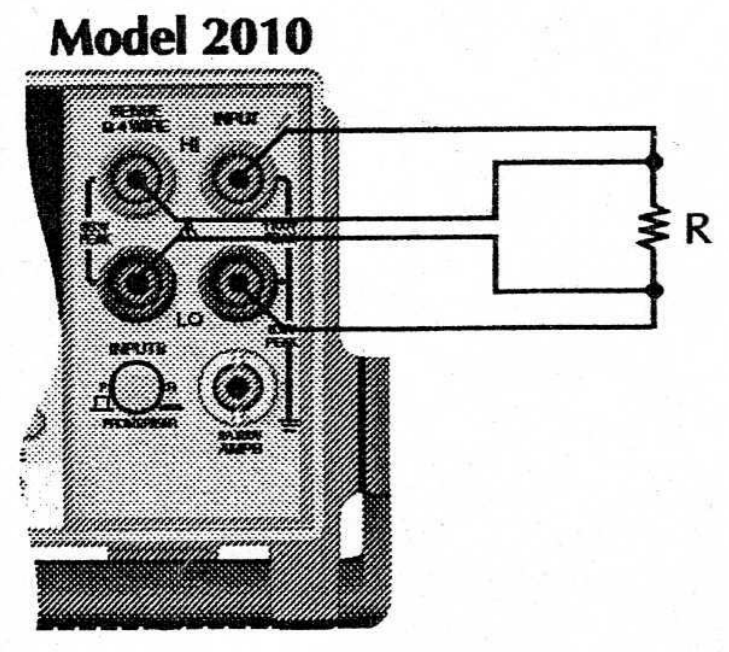
\includegraphics[scale=0.5]{keithley}
\caption{Znázornění měření multimetrem \textbf{KEITHLEY 2010} \cite{stud_text}}
\label{fig:keithley}
\end{figure}

Měrný odpor je definován vztahem 
\begin{equation} \label{eq:merny_odpor}
\rho = \frac{RS}{l} = \frac{R \pi d^2}{4l},
\end{equation}
kde $R$ je odpor homogenního vodiče délky $l$ a průměru $d$ s kruhovým průřezem.

V tabulkách je měrný elektrický odpor zpravidla uváděn pro teplotu $\SI{0}{\celsius}$ společně s hodnotou \textit{Teplotního součinitele odporu} $\alpha$. Pro danou teplotu $T$ spočteme měrný odpor podle
\begin{equation} \label{eq:odpor_teplota}
\rho(T) = \rho_0 (1 + \alpha T).
\end{equation}

\subsection*{Statistické vyhodnocení}
Průměrná hodnota naměřených veličin při $n$ měřeních je počítána podle vzorce aritmetického průměru 
\begin{equation}
\overline{x} = \frac{1}{n} \sum\limits_{i=1}^n{x_i}.
\end{equation}
Statistická chyba $\sigma_{stat}$ aritmetického průměru se získá ze vztahu 
\begin{equation}
\sigma_{stat} = \frac{\sqrt{\frac{1}{n-1} \sum\limits_{i=1}^n{(x_i - \overline{x})^2}}}{\sqrt{n}}.
\end{equation}
Absolutní chyba je potom získána z $\sigma_{stat}$ a chyby měřidla $\sigma_{\textit{měř}}$ jako 
\begin{equation}
\sigma = \sqrt{\sigma_{\textit{měř}}^2 + \sigma_{stat}^2}.
\end{equation}

Chyba výpočtů se řídí zákonem přenosu chyb.

\end{document}
